%\addtocontents{toc}{\protect\contentsline{chapter}{Appendix}{}}
%\addtocontents{toc}{\protect\contentsline{chapter}{\appendixtocname}{}}
%\addtocontents{toc}{\protect\contentsline{chapter}{}{}}
%\addtocontents{toc}{\contentsline{chapter}{Appendix}{}}
%\addcontentsline{file}{type}{text}
%\addtocontents{toc}{\protect\setcounter{tocdepth}{0}}
%\addtocontents{lof}{\protect\setcounter{tocdepth}{0}}
%\renewcommand{\appendixname}{Appendix}
%\addappheadtotoc
%\renewcommand{\appendixname}{Appendix}
%\renewcommand{\appendixtocname}{List of appendices}
\chapter{Neural Network Parameters}
\section{Nguyen–Widrow Weights Initialization} \label{algorithm_appendix_nguyen_widrow_weight_initialization}

\acs{ann} uses learning algorithms to train the weights and biases of the network. We normally choose random values as initial weights for the network. The random choice of initial weights and biases will affect the performance and efficiency of the learning algorithms. If the average performance of the algorithm is required, a test using several different sets of initial weights and biases will be carried out. Good choice of initial weights and biases in the training phase of the experiments greatly impact the performance of the network training. The chosen initial weights determine the starting point in the error landscape, which controls whether the learning process will end up in a local minimum or the global minimum. The easiest method is to select the weights randomly from suitable range such as between [-1.0 1.0] or minmax(input range). More sophisticated approach for selecting the initial weights for the network training is the Nguyen-Widrow weight initialization technique. \par
Nguyen-Widrow weight initialization technique calculates the interval from which the weights are taken in accordance with the number of input neurons and the number of hidden neurons \cite{Nguyen1990}. Nguyen-Widrow weight initialization algorithm is given in algorithm \ref{algorithm_nguyen_widrow}.

\begin{algorithm}
\caption{Nguyen-Widrow Weight Initialization Algorithm}
\label{algorithm_nguyen_widrow}
\begin{algorithmic}[1]
\STATE Calculate parameter $\beta$ using,\\
\STATE\qquad$\beta=0.7*p^{\frac{1}{n}}$\\
\STATE\qquad\qquad where $p=$ number of hidden units and
\STATE\qquad\qquad\qquad $\;\;n=$ number of input units
\STATE Calculate weight $w_{ij}$ as,
\STATE\qquad $w_{ij}=\beta*\dfrac{w_{ij}(random)}{\lVert w_j(random)\rVert}$
\end{algorithmic}
\end{algorithm}

\section{Activation Function}
\label{appendix_activation_functions}
A activation function (also known as transfer function) determines the relation between input and output. Activation function normalizes the output value to certain range. There are number of activation functions in use with neural networks. Activation functions may be linear or non-linear. Some of the widely used activation functions are McCulloch-Pitts thresholding function, piecewise-linear function and sigmoid function.

Sigmoid function has s-shaped graph and is most common form of activation function for defining the output of a neuron. Sigmoid function is strictly increasing, continuous and differential function. It exhibits a graceful balance between linear and nonlinear behavior. An example of the sigmoid function is the logistic function, defined by,
\begin{equation}
\phi(v)=\frac{1}{1+\exp(-av)}
\end{equation}
where, $a$ is the slope parameter of the sigmoid function and $v$ is the local output of the neuron.

Hyperbolic tangent sigmoid activation function is symmetric bipolar activation function, defined by,

\begin{equation}
\phi(v)=\frac{2}{(1+\exp(-2v))}-1
\end{equation}

The graph of hyperbolic tangent sigmoid activation function is given in figure \ref{figure_tanh_activation_function}.
\begin{figure}[h]
\centering
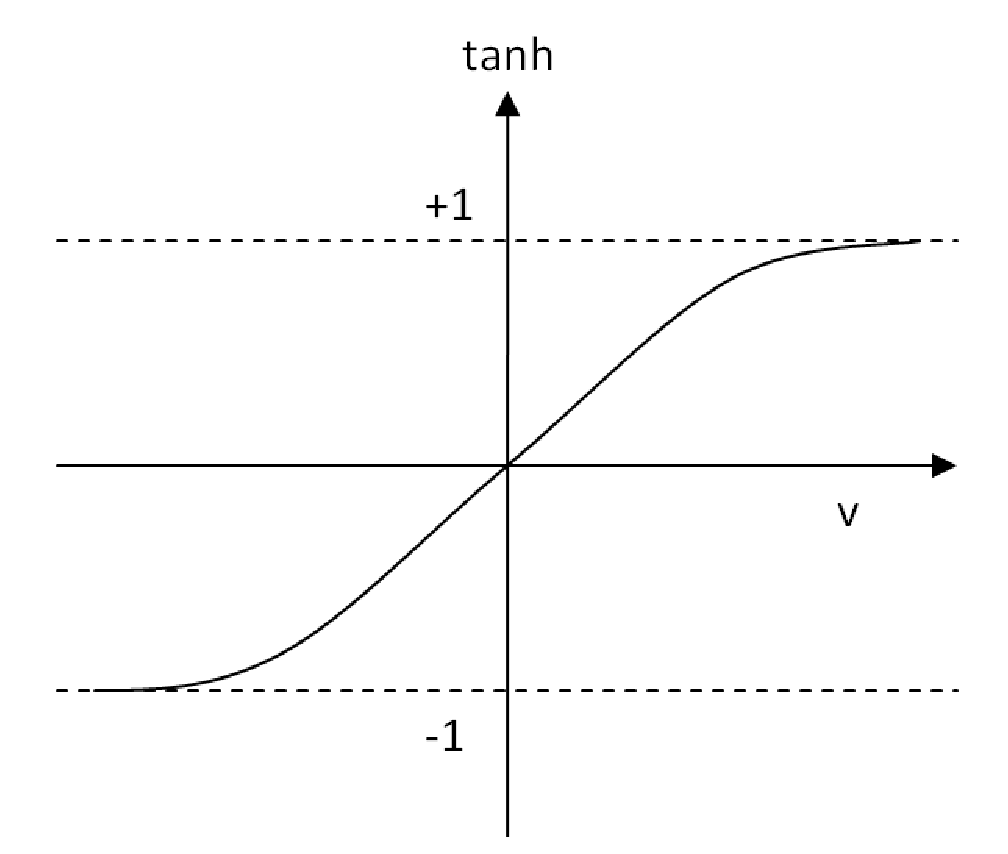
\includegraphics[width=4in]{figures/ann/tanh.eps}
\caption{Hyperbolic tangent sigmoid activation function.}
\label{figure_tanh_activation_function}
\end{figure}